\label{Section:Implementation}

The implementation follows the concept in the previous chapter, a detailed flow diagram of the application can be seen in Figure \ref{Figure:Application-StateMachine}. To be able to receive a trap while the application is running, a separate thread is needed. This can be seen in the figure, where the flow splits into two separate paths. If a terminating signal is received, both threads will get terminated.

The application is using snmpwalk to query data from devices. There is an open-source implementation of it by the net-snmp project. It is compiled by the build system and executed by \textit{exec} from the application. Its output is parsed by the application. A more clean way would be using a library and not executing a precompiled executable. A common library for that is net-snmp, but due to the broad platform and version support, it is very complex. For a first prototype, the precompiled executable has been used. This implementation will deliver the queried data as a string over stdout.

For the deep scan, the application is using onesixtyone \footnote{https://github.com/trailofbits/onesixtyone}. It is the most common open-source implementation for such a task. With it, it is possible to scan the network for SNMP devices in a very short time span. This program is precompiled, executed with \textit{exec} and the output parsed by the application.

Due to the usage of a precompiled version of \textit{snmpwalk}, the application needs to parse a lot of strings. Because string operations are limited in C, it was decided to use a dedicated library. The library sds has been selected for the application. Sds manages the memory allocation for the strings and is compatible with default C strings. The library also offers multiple methods, that are faster than the corresponding C string functions. It also offers functions that provide more comfort, e.g. tokenize a string with a specific delimiter. When using sds methods, the developer needs to be aware that the methods need to be used in other ways than default c \textit{string.h} methods.

To save the queried data in the structure needed, the application uses sqlite3 \footnote{https://www.sqlite.org/index.html}. Sqlite was selected because it is easy to use with C. The sqlite3 library has a simple API to create a database and execute SQL statements. With SQL it is possible to easily query data, with specific and complex conditions. Linking entries with others is possible, which makes it easy to represent connections. Sqlite has good portability, which means other applications can interact with the database easily. Data of a Sqlite database can easily be visualized using existing tools. This makes it easy to use in the development process and can be helpful with debugging. In Figure \ref{Figure:Concept-DatabaseSchema} the database schema that has been used can be seen.

\begin{figure}
\begin{center}
\begin{tikzpicture}[scale=0.8]
\node (Devices) [scale=0.8,shape=rectangle,draw,anchor=west] at (1, 10)
{
    \begin{tabular}{l|l|l}
        \multicolumn{3}{c}{{Devices}}\\
        \cmidrule(lr){1-3} & & \\
        id & INTEGER & PRIMARY KEY, AI\\
        ManagementAddress & INTEGER & \\
        CapabilitiesSupported & INTEGER & \\
        CapabilitiesEnabled & INTEGER & \\
        SystemName & TEXT & \\
    \end{tabular}
};
\node (Ports) [scale=0.8,shape=rectangle,draw,anchor=west] at (1, 5)
{
    \begin{tabular}{l|l|l}
        \multicolumn{3}{c}{{Ports}}\\
        \cmidrule(lr){1-3} & & \\
        id & INTEGER & PRIMARY KEY, AI\\
        DeviceId & INTEGER & FOREIGN KEY (Device.Id)\\
        InterfaceId & INTEGER & \\
        MACAddress & TEXT & \\
        MaxSpeed & INTEGER & \\
        OperatingStatus & INTEGER & \\
        Name & TEXT & \\
    \end{tabular}
};
\node (Links) [scale=0.8,shape=rectangle,draw,anchor=west] at (1, 0)
{
    \begin{tabular}{l|l|l}
        \multicolumn{3}{c}{{Links}}\\
        \cmidrule(lr){1-3} & & \\
        id & INTEGER & PRIMARY KEY, AI\\
        PortAId & INTEGER & FOREIGN KEY (Port.Id)\\
        PortBId & INTEGER & FOREIGN KEY (Port.Id)\\
        LinkType & INTEGER & \\
        Speed & INTEGER & \\
        Length & INTEGER & \\
    \end{tabular}
};

\draw (1,5.5) -- (0,5.5);
\draw (0,5.5) -- (0,10.5);
\draw [-{Latex[scale=1.5]}] (0,10.5) -- (1,10.5);

\draw (1, 0.2) -- (0.6, 0.2);
\draw (1,-0.3) -- (0.3,-0.3);
\draw (0.3,-0.3) -- (0.3,5.9);
\draw (0.6, 0.2) -- (0.6,5.9);
\draw [-{Latex[scale=1.5]}] (0.3,5.9) -- (1,5.9);

\end{tikzpicture}
\end{center}
\caption{Database schema visualization of the application.}
\label{Figure:Concept-DatabaseSchema}
\end{figure}

\begin{figure}
    \begin{adjustbox}{width=\textwidth}
    \tikzset{every picture/.style={line width=0.75pt}} %set default line width to 0.75pt        
    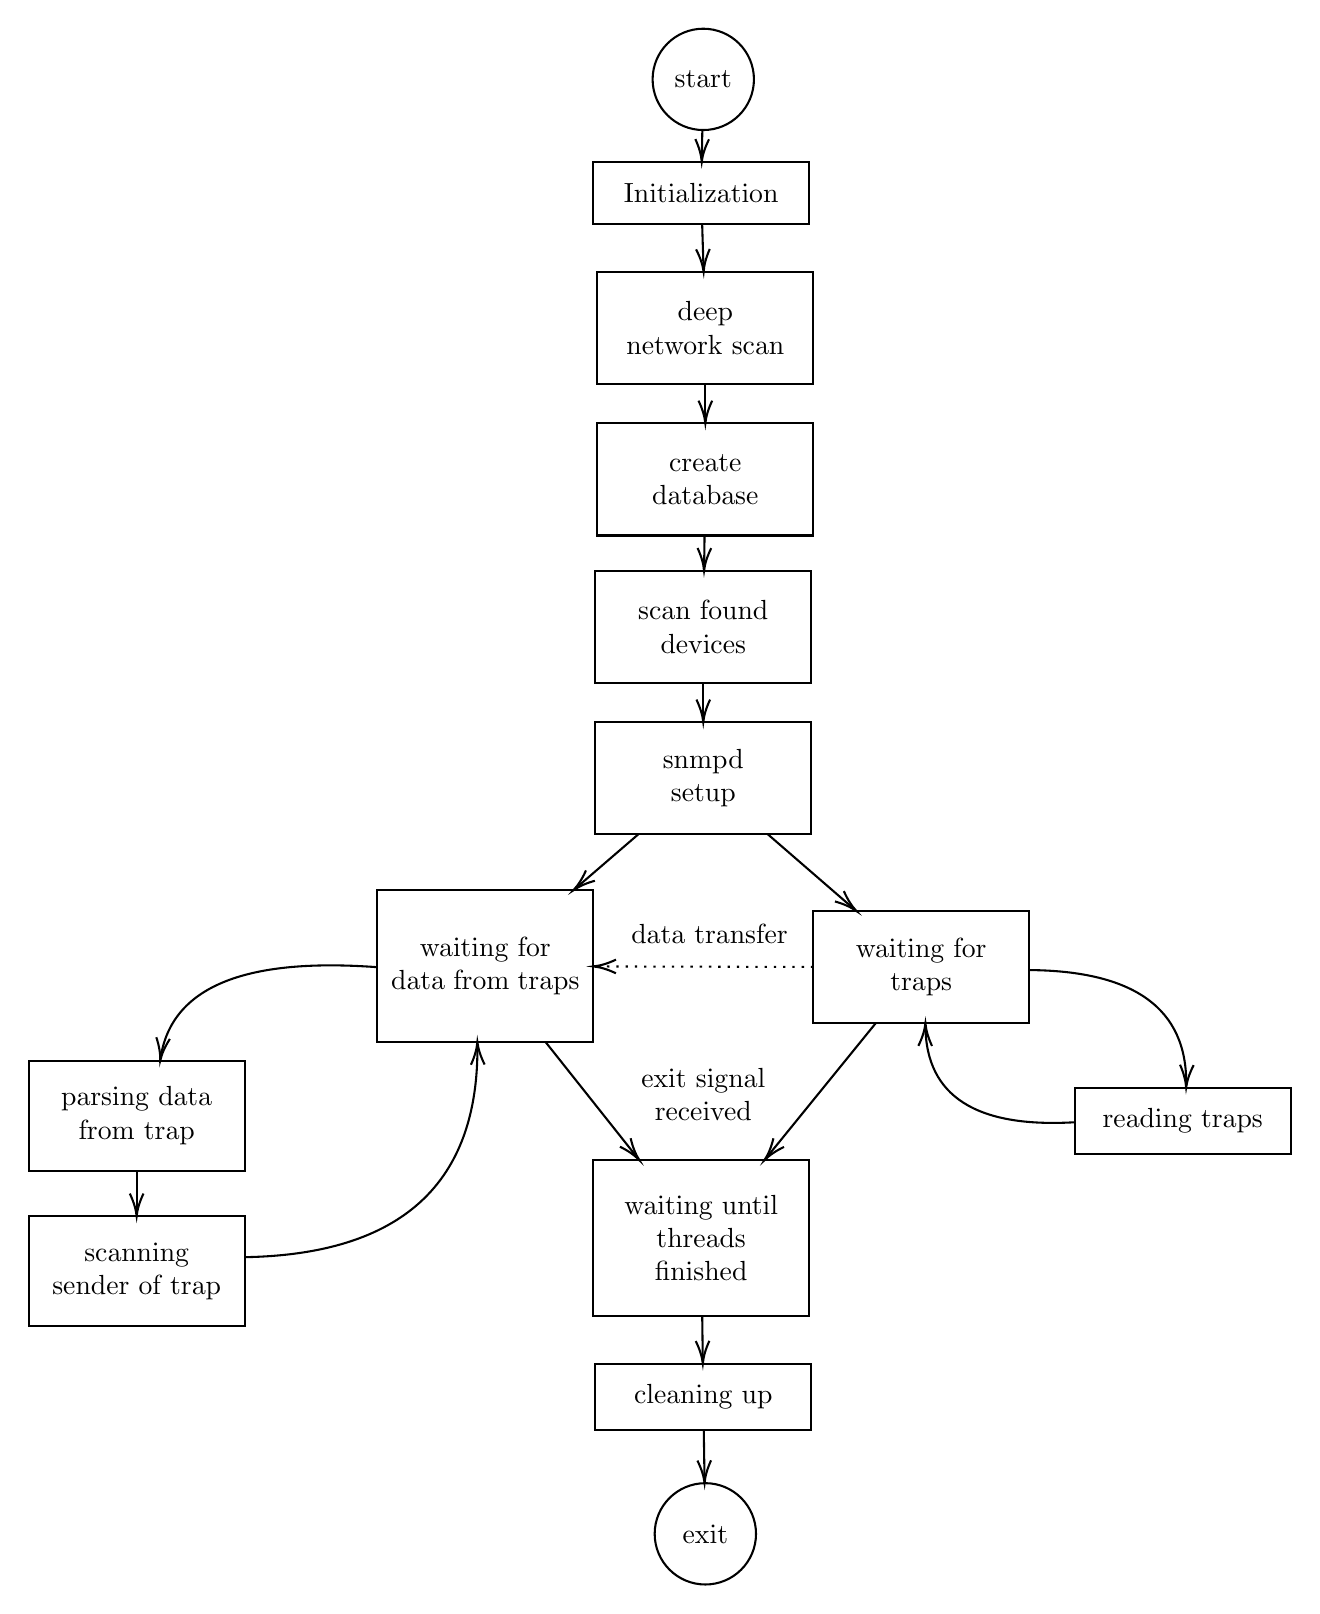
\begin{tikzpicture}[x=0.75pt,y=0.75pt,yscale=-1,xscale=1]
        %uncomment if require: \path (0,768); %set diagram left start at 0, and has height of 768
        
        % Text Node
        \draw    (304,65.75) -- (408,65.75) -- (408,95.75) -- (304,95.75) -- cycle  ;
        \draw (356,80.75) node   [align=left] {\begin{minipage}[lt]{68pt}\setlength\topsep{0pt}
        \begin{center}
        Initialization
        \end{center}
        
        \end{minipage}};
        % Text Node
        \draw    (306,118.75) -- (410,118.75) -- (410,172.75) -- (306,172.75) -- cycle  ;
        \draw (358,145.75) node   [align=left] {\begin{minipage}[lt]{68pt}\setlength\topsep{0pt}
        \begin{center}
        deep\\network scan
        \end{center}
        
        \end{minipage}};
        % Text Node
        \draw    (306,191.75) -- (410,191.75) -- (410,245.75) -- (306,245.75) -- cycle  ;
        \draw (358,218.75) node   [align=left] {\begin{minipage}[lt]{68pt}\setlength\topsep{0pt}
        \begin{center}
        create\\database
        \end{center}
        
        \end{minipage}};
        % Text Node
        \draw    (305,262.75) -- (409,262.75) -- (409,316.75) -- (305,316.75) -- cycle  ;
        \draw (357,289.75) node   [align=left] {\begin{minipage}[lt]{68pt}\setlength\topsep{0pt}
        \begin{center}
        scan found devices
        \end{center}
        
        \end{minipage}};
        % Text Node
        \draw    (305,335.75) -- (409,335.75) -- (409,389.75) -- (305,389.75) -- cycle  ;
        \draw (357,362.75) node   [align=left] {\begin{minipage}[lt]{68pt}\setlength\topsep{0pt}
        \begin{center}
        snmpd\\setup
        \end{center}
        
        \end{minipage}};
        % Text Node
        \draw    (410,426.75) -- (514,426.75) -- (514,480.75) -- (410,480.75) -- cycle  ;
        \draw (462,453.75) node   [align=left] {\begin{minipage}[lt]{68pt}\setlength\topsep{0pt}
        \begin{center}
        waiting for\\traps
        \end{center}
        
        \end{minipage}};
        % Text Node
        \draw    (200,416.75) -- (304,416.75) -- (304,489.75) -- (200,489.75) -- cycle  ;
        \draw (252,453.25) node   [align=left] {\begin{minipage}[lt]{68pt}\setlength\topsep{0pt}
        \begin{center}
        waiting for\\data from traps
        \end{center}
        
        \end{minipage}};
        % Text Node
        \draw    (32,498.75) -- (136,498.75) -- (136,551.75) -- (32,551.75) -- cycle  ;
        \draw (84,525.25) node   [align=left] {\begin{minipage}[lt]{68pt}\setlength\topsep{0pt}
        \begin{center}
        parsing data from trap
        \end{center}
        
        \end{minipage}};
        % Text Node
        \draw    (32,573.75) -- (136,573.75) -- (136,626.75) -- (32,626.75) -- cycle  ;
        \draw (84,600.25) node   [align=left] {\begin{minipage}[lt]{68pt}\setlength\topsep{0pt}
        \begin{center}
        scanning sender of trap
        \end{center}
        
        \end{minipage}};
        % Text Node
        \draw    (536,511.75) -- (640,511.75) -- (640,543.75) -- (536,543.75) -- cycle  ;
        \draw (588,527.75) node   [align=left] {\begin{minipage}[lt]{68pt}\setlength\topsep{0pt}
        \begin{center}
        reading traps
        \end{center}
        
        \end{minipage}};
        % Text Node
        \draw    (304,546.75) -- (408,546.75) -- (408,621.75) -- (304,621.75) -- cycle  ;
        \draw (356,584.25) node   [align=left] {\begin{minipage}[lt]{68pt}\setlength\topsep{0pt}
        \begin{center}
        waiting until threads finished
        \end{center}
        
        \end{minipage}};
        % Text Node
        \draw    (305,644.75) -- (409,644.75) -- (409,676.75) -- (305,676.75) -- cycle  ;
        \draw (357,660.75) node   [align=left] {\begin{minipage}[lt]{68pt}\setlength\topsep{0pt}
        \begin{center}
        cleaning up
        \end{center}
        
        \end{minipage}};
        % Text Node
        \draw    (358, 726.75) circle [x radius= 24.41, y radius= 24.41]   ;
        \draw (358,726.75) node   [align=left] {\begin{minipage}[lt]{25.84pt}\setlength\topsep{0pt}
        \begin{center}
        exit
        \end{center}
        
        \end{minipage}};
        % Text Node
        \draw    (357, 26) circle [x radius= 24.41, y radius= 24.41]   ;
        \draw (357,26) node   [align=left] {\begin{minipage}[lt]{25.84pt}\setlength\topsep{0pt}
        \begin{center}
        start
        \end{center}
        
        \end{minipage}};
        % Text Node
        \draw (357,515) node   [align=left] {\begin{minipage}[lt]{68pt}\setlength\topsep{0pt}
        \begin{center}
        exit signal\\received
        \end{center}
        
        \end{minipage}};
        % Text Node
        \draw (360,437.75) node   [align=left] {\begin{minipage}[lt]{68pt}\setlength\topsep{0pt}
        \begin{center}
        data transfer
        \end{center}
        
        \end{minipage}};
        % Connection
        \draw    (356.46,95.75) -- (357.11,116.75) ;
        \draw [shift={(357.17,118.75)}, rotate = 268.24] [color={rgb, 255:red, 0; green, 0; blue, 0 }  ][line width=0.75]    (10.93,-3.29) .. controls (6.95,-1.4) and (3.31,-0.3) .. (0,0) .. controls (3.31,0.3) and (6.95,1.4) .. (10.93,3.29)   ;
        % Connection
        \draw    (358,172.75) -- (358,189.75) ;
        \draw [shift={(358,191.75)}, rotate = 270] [color={rgb, 255:red, 0; green, 0; blue, 0 }  ][line width=0.75]    (10.93,-3.29) .. controls (6.95,-1.4) and (3.31,-0.3) .. (0,0) .. controls (3.31,0.3) and (6.95,1.4) .. (10.93,3.29)   ;
        % Connection
        \draw    (357.62,245.75) -- (357.41,260.75) ;
        \draw [shift={(357.38,262.75)}, rotate = 270.81] [color={rgb, 255:red, 0; green, 0; blue, 0 }  ][line width=0.75]    (10.93,-3.29) .. controls (6.95,-1.4) and (3.31,-0.3) .. (0,0) .. controls (3.31,0.3) and (6.95,1.4) .. (10.93,3.29)   ;
        % Connection
        \draw    (357,316.75) -- (357,333.75) ;
        \draw [shift={(357,335.75)}, rotate = 270] [color={rgb, 255:red, 0; green, 0; blue, 0 }  ][line width=0.75]    (10.93,-3.29) .. controls (6.95,-1.4) and (3.31,-0.3) .. (0,0) .. controls (3.31,0.3) and (6.95,1.4) .. (10.93,3.29)   ;
        % Connection
        \draw    (388.15,389.75) -- (429.33,425.44) ;
        \draw [shift={(430.85,426.75)}, rotate = 220.91] [color={rgb, 255:red, 0; green, 0; blue, 0 }  ][line width=0.75]    (10.93,-3.29) .. controls (6.95,-1.4) and (3.31,-0.3) .. (0,0) .. controls (3.31,0.3) and (6.95,1.4) .. (10.93,3.29)   ;
        % Connection
        \draw    (325.67,389.75) -- (295.86,415.44) ;
        \draw [shift={(294.35,416.75)}, rotate = 319.24] [color={rgb, 255:red, 0; green, 0; blue, 0 }  ][line width=0.75]    (10.93,-3.29) .. controls (6.95,-1.4) and (3.31,-0.3) .. (0,0) .. controls (3.31,0.3) and (6.95,1.4) .. (10.93,3.29)   ;
        % Connection
        \draw    (440.07,480.75) -- (387.72,545.2) ;
        \draw [shift={(386.46,546.75)}, rotate = 309.09] [color={rgb, 255:red, 0; green, 0; blue, 0 }  ][line width=0.75]    (10.93,-3.29) .. controls (6.95,-1.4) and (3.31,-0.3) .. (0,0) .. controls (3.31,0.3) and (6.95,1.4) .. (10.93,3.29)   ;
        % Connection
        \draw    (280.98,489.75) -- (324.99,545.18) ;
        \draw [shift={(326.23,546.75)}, rotate = 231.55] [color={rgb, 255:red, 0; green, 0; blue, 0 }  ][line width=0.75]    (10.93,-3.29) .. controls (6.95,-1.4) and (3.31,-0.3) .. (0,0) .. controls (3.31,0.3) and (6.95,1.4) .. (10.93,3.29)   ;
        % Connection
        \draw    (356.49,621.75) -- (356.76,642.75) ;
        \draw [shift={(356.79,644.75)}, rotate = 269.25] [color={rgb, 255:red, 0; green, 0; blue, 0 }  ][line width=0.75]    (10.93,-3.29) .. controls (6.95,-1.4) and (3.31,-0.3) .. (0,0) .. controls (3.31,0.3) and (6.95,1.4) .. (10.93,3.29)   ;
        % Connection
        \draw    (357.24,676.75) -- (357.6,700.34) ;
        \draw [shift={(357.63,702.34)}, rotate = 269.13] [color={rgb, 255:red, 0; green, 0; blue, 0 }  ][line width=0.75]    (10.93,-3.29) .. controls (6.95,-1.4) and (3.31,-0.3) .. (0,0) .. controls (3.31,0.3) and (6.95,1.4) .. (10.93,3.29)   ;
        % Connection
        \draw    (200,453.75) .. controls (135.65,448.98) and (100.84,463.46) .. (95.59,497.2) ;
        \draw [shift={(95.37,498.75)}, rotate = 277.23] [color={rgb, 255:red, 0; green, 0; blue, 0 }  ][line width=0.75]    (10.93,-3.29) .. controls (6.95,-1.4) and (3.31,-0.3) .. (0,0) .. controls (3.31,0.3) and (6.95,1.4) .. (10.93,3.29)   ;
        % Connection
        \draw    (514,455.13) .. controls (564.8,455.49) and (590.02,473.81) .. (589.68,510.08) ;
        \draw [shift={(589.65,511.75)}, rotate = 271.74] [color={rgb, 255:red, 0; green, 0; blue, 0 }  ][line width=0.75]    (10.93,-3.29) .. controls (6.95,-1.4) and (3.31,-0.3) .. (0,0) .. controls (3.31,0.3) and (6.95,1.4) .. (10.93,3.29)   ;
        % Connection
        \draw    (536,528.45) .. controls (488.38,531.25) and (464.39,515.86) .. (464.04,482.3) ;
        \draw [shift={(464.04,480.75)}, rotate = 90.62] [color={rgb, 255:red, 0; green, 0; blue, 0 }  ][line width=0.75]    (10.93,-3.29) .. controls (6.95,-1.4) and (3.31,-0.3) .. (0,0) .. controls (3.31,0.3) and (6.95,1.4) .. (10.93,3.29)   ;
        % Connection
        \draw    (84,551.75) -- (84,571.75) ;
        \draw [shift={(84,573.75)}, rotate = 270] [color={rgb, 255:red, 0; green, 0; blue, 0 }  ][line width=0.75]    (10.93,-3.29) .. controls (6.95,-1.4) and (3.31,-0.3) .. (0,0) .. controls (3.31,0.3) and (6.95,1.4) .. (10.93,3.29)   ;
        % Connection
        \draw    (136,593.46) .. controls (211.62,592.16) and (249.02,557.92) .. (248.17,490.76) ;
        \draw [shift={(248.16,489.75)}, rotate = 88.96] [color={rgb, 255:red, 0; green, 0; blue, 0 }  ][line width=0.75]    (10.93,-3.29) .. controls (6.95,-1.4) and (3.31,-0.3) .. (0,0) .. controls (3.31,0.3) and (6.95,1.4) .. (10.93,3.29)   ;
        % Connection
        \draw    (356.55,50.41) -- (356.31,63.75) ;
        \draw [shift={(356.27,65.75)}, rotate = 271.05] [color={rgb, 255:red, 0; green, 0; blue, 0 }  ][line width=0.75]    (10.93,-3.29) .. controls (6.95,-1.4) and (3.31,-0.3) .. (0,0) .. controls (3.31,0.3) and (6.95,1.4) .. (10.93,3.29)   ;
        % Connection
        \draw  [dash pattern={on 0.84pt off 2.51pt}]  (410,453.63) -- (306,453.38) ;
        \draw [shift={(304,453.37)}, rotate = 0.14] [color={rgb, 255:red, 0; green, 0; blue, 0 }  ][line width=0.75]    (10.93,-3.29) .. controls (6.95,-1.4) and (3.31,-0.3) .. (0,0) .. controls (3.31,0.3) and (6.95,1.4) .. (10.93,3.29)   ;
    \end{tikzpicture}
    \end{adjustbox}
    \caption{Program flow of the application.}
    \label{Figure:Application-StateMachine}
\end{figure} 

